\documentclass[tikz]{standalone}
\usetikzlibrary{arrows, positioning}
\tikzset{
  treenode/.style = {align=center, inner sep=1pt, text centered,
    font=\sffamily},
  bst/.style = {treenode, circle, black, font=\sffamily\bfseries, draw=black, text width=2em}, 
  sst/.style = {treenode, circle, black, font=\sffamily\bfseries, draw=red, text width=2em}, 
  txt/.style = {text width=1.5em, red},
  redline/.style={edge from parent/.style={red,very thick,latex-, draw}},
  rugularline/.style={edge from parent/.style={black, line width=0.2mm, draw}},
}
\begin{document}
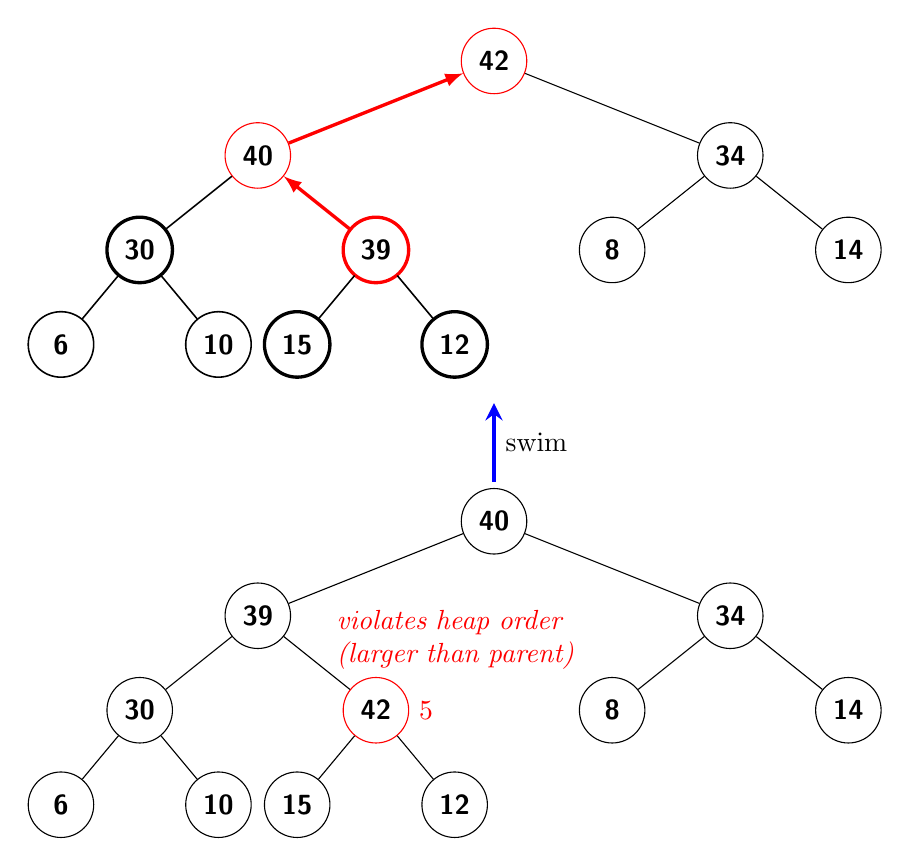
\begin{tikzpicture}[level/.style={sibling distance = 6cm/#1,
  level distance = 1.2cm}]
\node [bst] (n1) {40}
    child {node [bst] {39}
        child {node [bst] {30}
            child {node [bst] {6}}
            child {node [bst] {10}}
        }
        child {node (n5) [sst] {42}
            child {node [bst] {15}}
            child {node [bst] {12}}
        }
    }
    child { node [bst] {34}
        child{node [bst] {8}}
        child{node [bst] {14}}
    }
;
\node [right, txt] at (n5.east) {5};
\node [below, txt, text width=4cm, yshift=-1cm] at (n1) {\textit{violates heap order \\(larger than parent)}};

\draw [-stealth, line width=0.6mm, draw=blue](0,0.5) -- (0,1.5)node[midway,right,shape=rectangle,draw=none]{swim};

\node [sst, above=of n1, yshift=4cm] (2n1) {42}
    child [redline] {node [sst] {40}
        child [rugularline] {node [bst] {30}
            child [rugularline] {node [bst] {6}}
            child [rugularline] {node [bst] {10}}
        }
        child {node (2n5) [sst] {39}
            child [rugularline] {node [bst] {15}}
            child [rugularline] {node [bst] {12}}
        }
    }
    child { node [bst] {34}
        child{node [bst] {8}}
        child{node [bst] {14}}
    }
;

\end{tikzpicture}
\end{document}
